\section{Aim}
 To study about various data constraints and views in SQL.

\section{{Theory}}

\subsection{Data Constraints}

The following are commonly used constraints available in PostgreSQL.
\begin{itemize}
    \item NOT NULL Constraint - Ensures that a column cannot have NULL value.
    \item UNIQUE Constraint - Ensures that all values in a column are different.
    \item PRIMARY Key - Uniquely identifies each row/record in a database table.
    \item FOREIGN Key - Constrains data based on columns in other tables.
    \item CHECK Constraint - The CHECK constraint ensures that all values in a column satisfy certain conditions.
\end{itemize}

\subsection{Views}

Views are pseudo-tables. That is, they are not real tables, but they appear as ordinary tables to SELECT. A view can represent a subset of a real table, selecting certain columns or certain rows from an ordinary table. A view can even represent joined tables. Because views are assigned separate permissions, you can use them to restrict table access so that the users see only specific rows or columns of a table.

\subsubsection{Syntax}

\begin{minted}{sql}
CREATE [TEMP | TEMPORARY] VIEW view_name AS
SELECT column1, column2.....
FROM table_name
WHERE [condition];
\end{minted}

\section{{Code and Output}}

\begin{enumerate}
\item
\begin{enumerate}
\item Create a table named Subjects with the given attributes
\begin{itemize}
\item Subid( Should not be NULL)
\item Subname (Should not be NULL)
\end{itemize}
Populate the database. Make sure that all constraints are working properly.\newline
\begin{minted}{sql}

CREATE TABLE subjects(
	subid int not null,
	subname char(20) not null
	);

INSERT INTO subjects VALUES(1, 'Maths');
INSERT INTO subjects VALUES(1, 'Physics');
INSERT INTO subjects VALUES(1, 'Chemistry');
INSERT INTO subjects VALUES(1, 'English');


\end{minted}
\newline
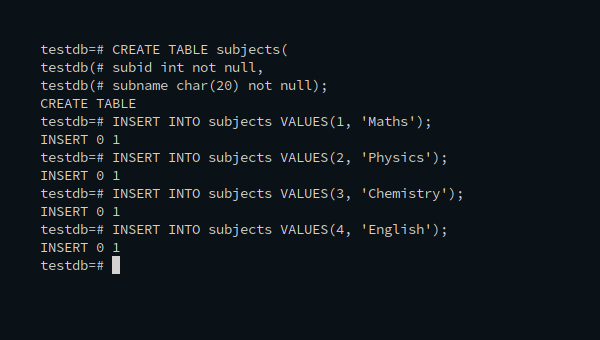
\includegraphics[width=\linewidth]{../Images/Constraints/1.png}\newline
\begin{enumerate}
\item Alter the table to set subid as the primary key.\newline
\begin{minted}{sql}

ALTER TABLE subjects ADD CONSTRAINT 
	pk PRIMARY KEY(subid);

\end{minted}
\newline
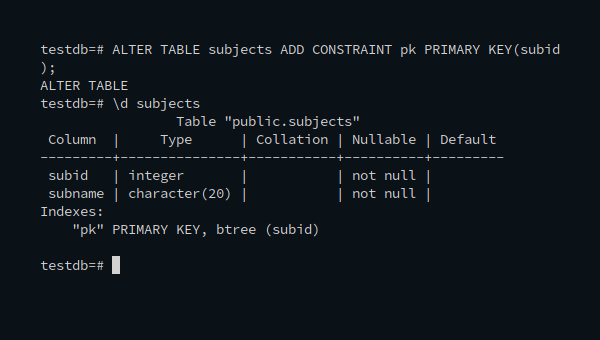
\includegraphics[width=\linewidth]{../Images/Constraints/2.png}\newline
\end{enumerate}
\item Create a table named Staff with the given attributes:
\begin{itemize}
\item staffid (Should be UNIQUE)
\item staffname
\item dept
\item age (Greater than 22)
\item salary (Less than 35000)
\end{itemize}
Populate the database. Make sure that all constraints are working properly.\newline
\begin{minted}{sql}

CREATE TABLE staff(
	staffid int unique,
	staffname char(20),
	delt char(15),
	age int check(age > 22),
	salary int check(salary < 35000)
	);
INSERT INTO staff 
	VALUES(1, 'John', 'Purchasing', 24, 30000);

INSERT INTO staff 
	VALUES(2, 'Sera', 'Sales', 25, 20000);
	
INSERT INTO staff 
	VALUES(3, 'John', 'Sales', 28, 25000);

\end{minted}
\newline
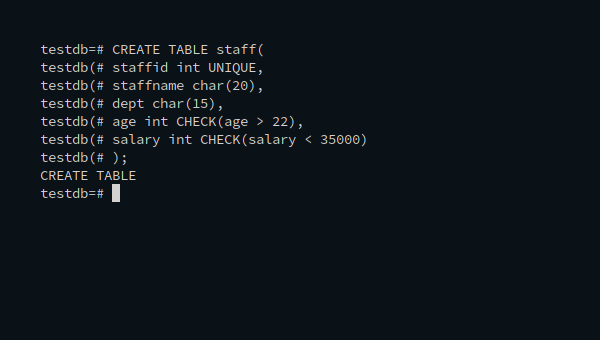
\includegraphics[width=\linewidth]{../Images/Constraints/3.png}\newline
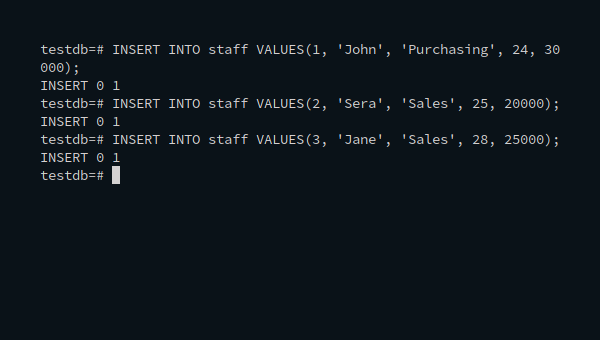
\includegraphics[width=\linewidth]{../Images/Constraints/4.png}\newline
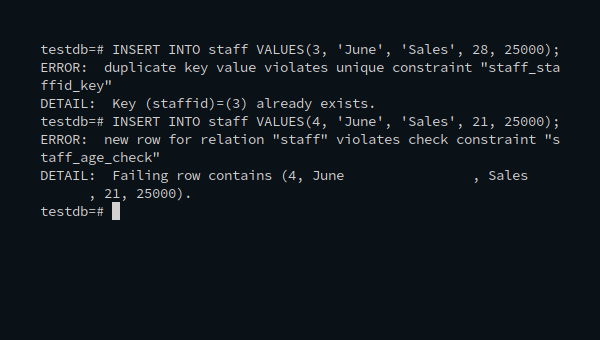
\includegraphics[width=\linewidth]{../Images/Constraints/5.png}\newline
\begin{enumerate}
\item Delete the check constraint imposed on the attribute salary\newline
\begin{minted}{sql}

ALTER TABLE staff 
	DROP CONSTRAINT staff_salary_check;

\end{minted}
\newline
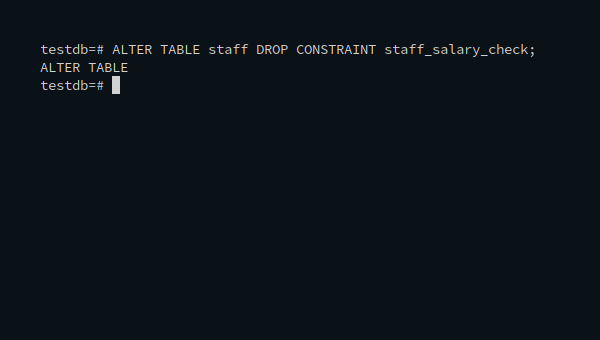
\includegraphics[width=\linewidth]{../Images/Constraints/6.png}\newline
\item Delete the unique constraint on the attribute staffid\newline
\begin{minted}{sql}

ALTER TABLE staff 
	DROP CONSTRAINT staff_salary_key;

\end{minted}
\newline
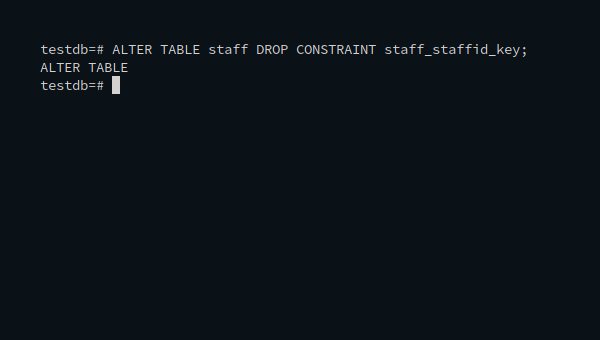
\includegraphics[width=\linewidth]{../Images/Constraints/7.png}\newline
\end{enumerate}
\item Create a table named Bank with the following attributes
\begin{itemize}
\item bankcode (To be set as Primary Key, type= varchar(3) )
\item bankname (Should not be NULL)
\item headoffice
\item branches (Integer value greater than Zero)
\end{itemize}
Populate the database. Make sure that all constraints are working properly.All constraints have to be set after creating the table.\newline
\begin{minted}{sql}

CREATE TABLE bank(
	bankcode varchar(3),
	bankname varchar(10),
	headoffice varchar(10),
	branches int
	);
ALTER TABLE bank 
	ADD CONSTRAINT bank_pk PRIMARY KEY(bankcode),
	ADD CONSTRAINT bnk_bankname_not_null 
		CHECK bankname IS NOT NULL),
	ADD CONSTRAINT bank_branches_check 
		CHECK(branches > 0);

\end{minted}
\newline
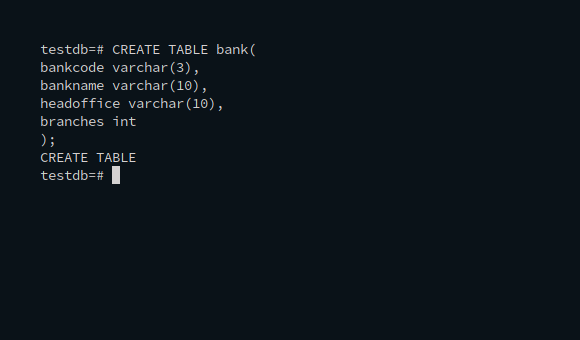
\includegraphics[width=\linewidth]{../Images/Constraints/8.png}\newline
\newline
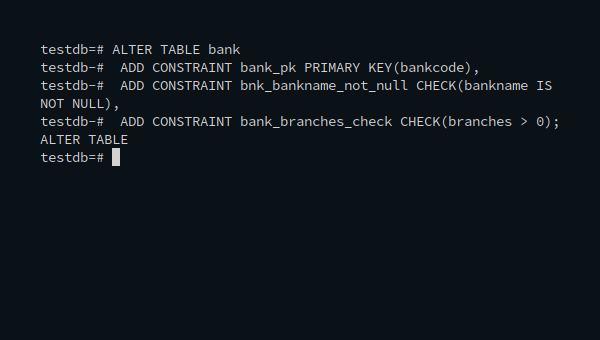
\includegraphics[width=\linewidth]{../Images/Constraints/9.png}\newline
\newline
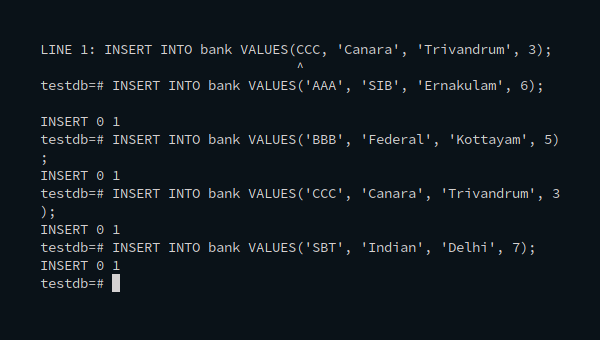
\includegraphics[width=\linewidth]{../Images/Constraints/10.png}\newline
\item Create a table named Branch with the following attributes
\begin{itemize}
\item branchid (To be set as Primary Key)
\item branchname (Set Default value as ‘New Delhi’)
\item bankid (Foreign Key:- Refers to bank code of Bank table)
\end{itemize}
\begin{enumerate}
\item Populate the database. Make sure that all constraints are working properly.\newline
\begin{minted}{sql}

CREATEA TABLE branch(
	branchid PRIMARY KEY,
	branchname varchar(10) DEFAULT 'New Delhi',
	bankid varchar(10) 
		REFERENCES bank(bankcode)
		ON DELETE CASCADE
	);

\end{minted}
\newline
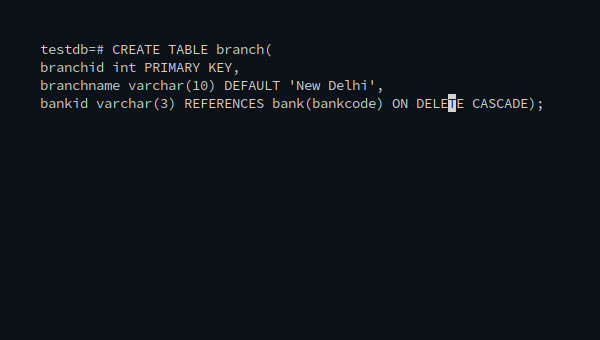
\includegraphics[width=\linewidth]{../Images/Constraints/11.png}\newline
\item During database population, demonstrate how the DEFAULT Constraint is satisfied.\newline
\begin{minted}{sql}

INSERT INTO branch(branchid, bankid) VALUES (02, 'AAA');

\end{minted}
\newline
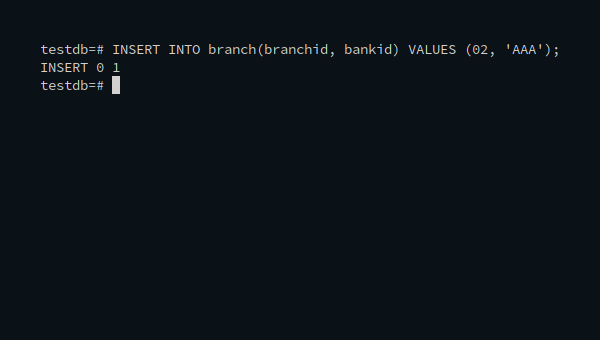
\includegraphics[width=\linewidth]{../Images/Constraints/12.png}\newline
\item Delete the bank with bank code ‘SBT’ and make sure that the corresponding entries are getting deleted from the related tables.\newline
\begin{minted}{sql}

DELETE FROM bank WHERE bankcode = 'SBT';

\end{minted}
\newline
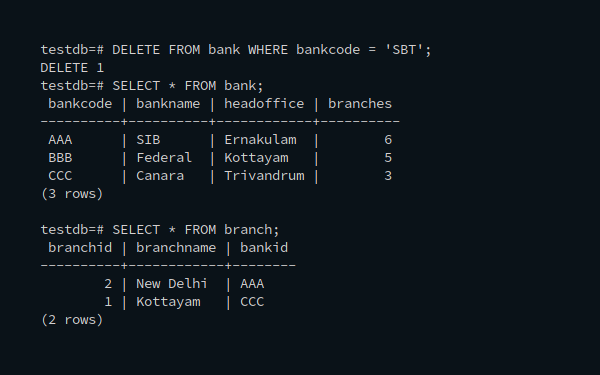
\includegraphics[width=\linewidth]{../Images/Constraints/13.png}\newline
\item Drop the Primary Key using ALTER command\newline
\begin{minted}{sql}

ALTER TABLE branch DROP CONSTRAINT branch_pkey;

\end{minted}
\newline
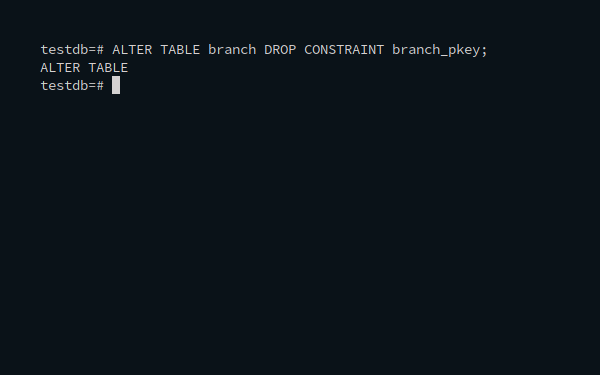
\includegraphics[width=\linewidth]{../Images/Constraints/14.png}\newline
\end{enumerate}
\end{enumerate}
\item Create a View named sales\_staff to hold the details of all staff working in sales Department\newline
\begin{minted}{sql}

CREATE VIEW sales_dept AS
	SELECT * FROM staff WHERE dept='Sales';

\end{minted}
\newline
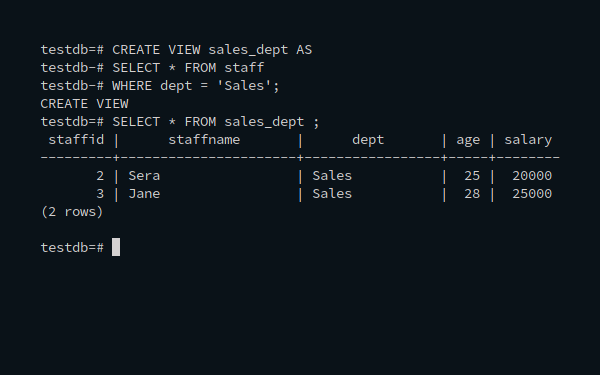
\includegraphics[width=\linewidth]{../Images/Constraints/15.png}\newline

\item Drop table branch. Create another table named branch and name all the constraints as given below:
\begin{itemize}
\item Constraint name Column Constraint
\item Pk branch\_id Primary key
\item Df branch\_name Default :’New Delhi’
\item Fk bankid Foreign key/References
\end{itemize}
\begin{minted}{sql}

DROP TABLE branch;
CREATE TABLE branch(
	branchid int,
	branchname varchar(10),
	bankid varchar(3)
	);
ALTER TABLE branch
	ADD CONSTRAINT Pk PRIMARY KEY(branchid),
	ADD CONSTRAINT Fk FOREIGN KEY(bankid) 
		REFERENCES bank(bankcode)
ALTER TABLE branch ALTER COLUMN branchname 
	SET DEFAULT 'New Delhi';

\end{minted}
\newline
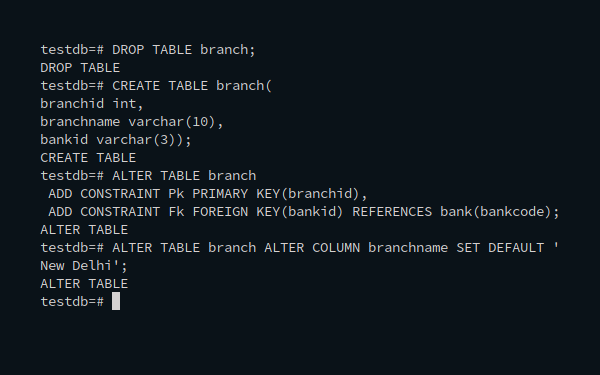
\includegraphics[width=\linewidth]{../Images/Constraints/16.png}\newline
\begin{enumerate}
\item Delete the default constraint in the table\newline
\begin{minted}{sql}

ALTER TABLE branch ALTER COLUMN branchname DROP DEFAULT;

\end{minted}
\newline
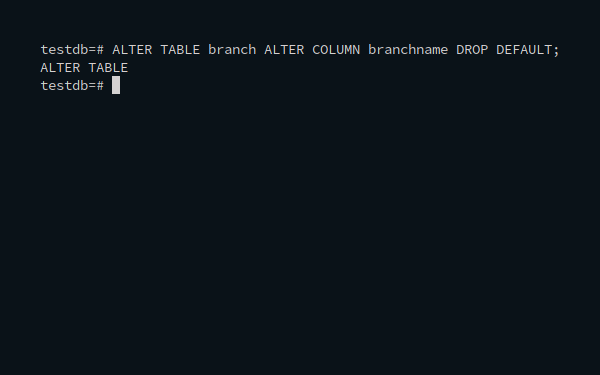
\includegraphics[width=\linewidth]{../Images/Constraints/17.png}\newline
\item Delete the primary key constraint\newline
\begin{minted}{sql}

ALTER TABLE branch DROP CONSTRAINT Pk;

\end{minted}
\newline
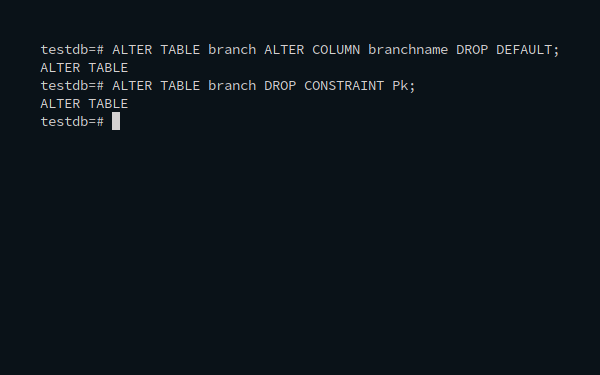
\includegraphics[width=\linewidth]{../Images/Constraints/18.png}\newline
\end{enumerate}

\item Update the view sales\_staff to include the details of staff belonging to sales department whose salary is greater than 20000.\newline
\begin{minted}{sql}

INSERT INTO staff VALUES(3, 'Jane', 'Sales', 28, 25000);

\end{minted}
\newline
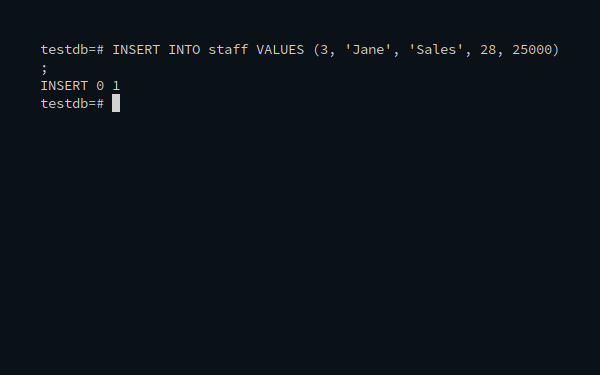
\includegraphics[width=\linewidth]{../Images/Constraints/19.png}\newline
\item Delete the view sales\_staff.\newline
\begin{minted}{sql}

DROP VIEW sales_dept;

\end{minted}
\newline
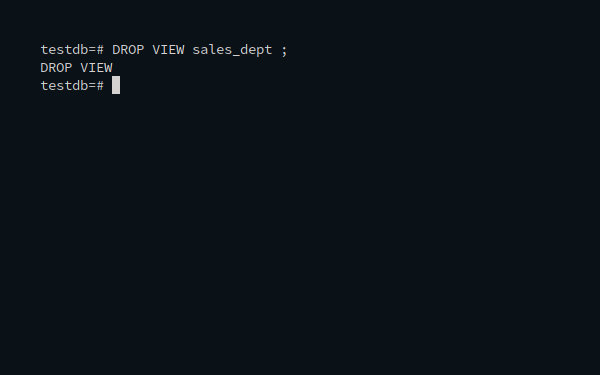
\includegraphics[width=\linewidth]{../Images/Constraints/20.png}\newline

\end{enumerate}



\section{Result}
Implemented the program for Data Constraints and Views using Postgresql 11.5 on Manjaro Linux and the output was obtained.